\hypertarget{LinearStatistic_8c}{
\section{LinearStatistic.c File Reference}
\label{LinearStatistic_8c}\index{LinearStatistic.c@{LinearStatistic.c}}
}
{\tt \#include \char`\"{}party.h\char`\"{}}\par


Include dependency graph for LinearStatistic.c:\nopagebreak
\begin{figure}[H]
\begin{center}
\leavevmode
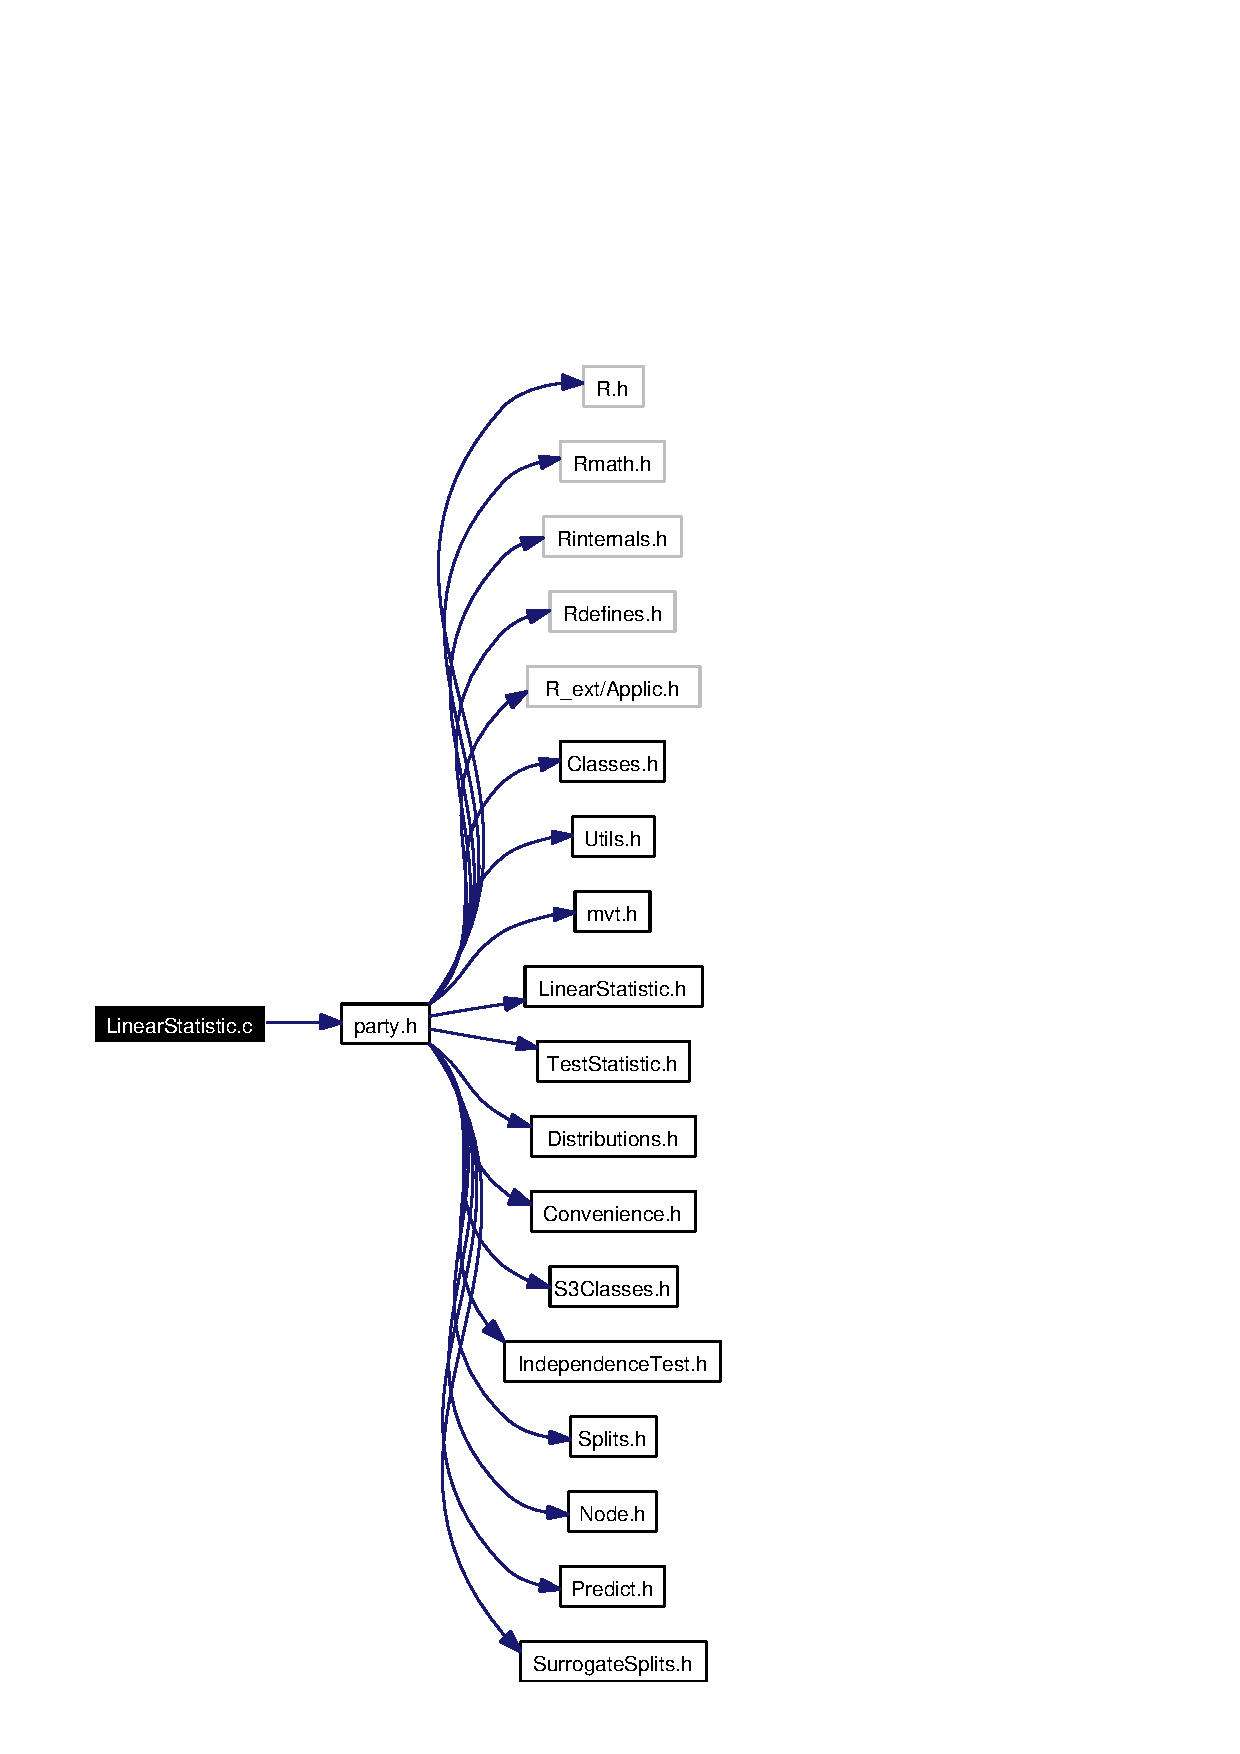
\includegraphics[width=420pt]{LinearStatistic_8c__incl}
\end{center}
\end{figure}
\subsection*{Functions}
\begin{CompactItemize}
\item 
void \hyperlink{LinearStatistic_8c_aefa2a9406bb30b323715e3db41da637}{C\_\-LinearStatistic} (const double $\ast$x, const int p, const double $\ast$y, const int q, const double $\ast$weights, const int n, double $\ast$ans)
\item 
SEXP \hyperlink{LinearStatistic_8c_732bfc8e1797d8953482aa31f9b43e5f}{R\_\-LinearStatistic} (SEXP x, SEXP y, SEXP weights)
\item 
void \hyperlink{LinearStatistic_8c_e2f62abe13ee5b625141b5d4a496d832}{C\_\-ExpectCovarInfluence} (const double $\ast$y, const int q, const double $\ast$weights, const int n, SEXP ans)
\item 
SEXP \hyperlink{LinearStatistic_8c_6216ea560644c08002fb32756ae67dcc}{R\_\-ExpectCovarInfluence} (SEXP y, SEXP weights)
\item 
void \hyperlink{LinearStatistic_8c_94a0805ea258af79d426c095feee399a}{C\_\-ExpectCovarLinearStatistic} (const double $\ast$x, const int p, const double $\ast$y, const int q, const double $\ast$weights, const int n, const SEXP expcovinf, SEXP ans)
\item 
SEXP \hyperlink{LinearStatistic_8c_58fff8082d3ab197994a21a10c422353}{R\_\-ExpectCovarLinearStatistic} (SEXP x, SEXP y, SEXP weights, SEXP expcovinf)
\item 
void \hyperlink{LinearStatistic_8c_a34b0f12fac36231a105d6dc903bfe89}{C\_\-PermutedLinearStatistic} (const double $\ast$x, const int p, const double $\ast$y, const int q, const int n, const int nperm, const int $\ast$indx, const int $\ast$perm, double $\ast$ans)
\item 
SEXP \hyperlink{LinearStatistic_8c_be383bcae17e8b3a1d5740ec16a9817a}{R\_\-PermutedLinearStatistic} (SEXP x, SEXP y, SEXP indx, SEXP perm)
\end{CompactItemize}


\subsection{Detailed Description}
Linear statistics for conditional inference based on Strasser \& Weber (1999)

\begin{Desc}
\item[Author:]\end{Desc}
\begin{Desc}
\item[Author]hothorn \end{Desc}
\begin{Desc}
\item[Date:]\end{Desc}
\begin{Desc}
\item[Date]2006-08-25 10:53:10 +0200 (Fri, 25 Aug 2006) \end{Desc}


Definition in file \hyperlink{LinearStatistic_8c-source}{LinearStatistic.c}.

\subsection{Function Documentation}
\hypertarget{LinearStatistic_8c_e2f62abe13ee5b625141b5d4a496d832}{
\index{LinearStatistic.c@{LinearStatistic.c}!C\_\-ExpectCovarInfluence@{C\_\-ExpectCovarInfluence}}
\index{C\_\-ExpectCovarInfluence@{C\_\-ExpectCovarInfluence}!LinearStatistic.c@{LinearStatistic.c}}
\subsubsection{\setlength{\rightskip}{0pt plus 5cm}void C\_\-ExpectCovarInfluence (const double $\ast$ {\em y}, \/  const int {\em q}, \/  const double $\ast$ {\em weights}, \/  const int {\em n}, \/  SEXP {\em ans})}}
\label{LinearStatistic_8c_e2f62abe13ee5b625141b5d4a496d832}


Conditional expectation and covariance of the influence function\par
 \begin{Desc}
\item[Parameters:]
\begin{description}
\item[{\em y}]values of the influence function \item[{\em q}]dimension of the influence function \item[{\em weights}]case weights \item[{\em n}]number of observations \item[{\em ans}]return value; an object of class `ExpectCovarInfluence' \end{description}
\end{Desc}


Definition at line 101 of file LinearStatistic.c.

References PL2\_\-covarianceSym, PL2\_\-expectationSym, and PL2\_\-sumweightsSym.

Referenced by C\_\-GlobalTest(), C\_\-LinStatExpCov(), C\_\-surrogates(), and R\_\-ExpectCovarInfluence().\hypertarget{LinearStatistic_8c_94a0805ea258af79d426c095feee399a}{
\index{LinearStatistic.c@{LinearStatistic.c}!C\_\-ExpectCovarLinearStatistic@{C\_\-ExpectCovarLinearStatistic}}
\index{C\_\-ExpectCovarLinearStatistic@{C\_\-ExpectCovarLinearStatistic}!LinearStatistic.c@{LinearStatistic.c}}
\subsubsection{\setlength{\rightskip}{0pt plus 5cm}void C\_\-ExpectCovarLinearStatistic (const double $\ast$ {\em x}, \/  const int {\em p}, \/  const double $\ast$ {\em y}, \/  const int {\em q}, \/  const double $\ast$ {\em weights}, \/  const int {\em n}, \/  const SEXP {\em expcovinf}, \/  SEXP {\em ans})}}
\label{LinearStatistic_8c_94a0805ea258af79d426c095feee399a}


Conditional expectation and covariance of the a linear statistic\par
 \begin{Desc}
\item[Parameters:]
\begin{description}
\item[{\em x}]values of the transformation \item[{\em p}]dimension of the transformation \item[{\em y}]values of the influence function \item[{\em q}]dimension of the influence function \item[{\em weights}]case weights \item[{\em n}]number of observations \item[{\em expcovinf}]an object of class `ExpectCovarInfluence' \item[{\em ans}]return value; an object of class `ExpectCovar' \end{description}
\end{Desc}


Definition at line 213 of file LinearStatistic.c.

References C\_\-kronecker(), PL2\_\-covarianceSym, PL2\_\-expectationSym, and PL2\_\-sumweightsSym.

Referenced by C\_\-LinStatExpCov(), and R\_\-ExpectCovarLinearStatistic().

Here is the call graph for this function:\nopagebreak
\begin{figure}[H]
\begin{center}
\leavevmode
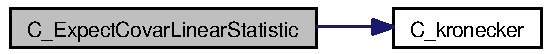
\includegraphics[width=150pt]{LinearStatistic_8c_94a0805ea258af79d426c095feee399a_cgraph}
\end{center}
\end{figure}
\hypertarget{LinearStatistic_8c_aefa2a9406bb30b323715e3db41da637}{
\index{LinearStatistic.c@{LinearStatistic.c}!C\_\-LinearStatistic@{C\_\-LinearStatistic}}
\index{C\_\-LinearStatistic@{C\_\-LinearStatistic}!LinearStatistic.c@{LinearStatistic.c}}
\subsubsection{\setlength{\rightskip}{0pt plus 5cm}void C\_\-LinearStatistic (const double $\ast$ {\em x}, \/  const int {\em p}, \/  const double $\ast$ {\em y}, \/  const int {\em q}, \/  const double $\ast$ {\em weights}, \/  const int {\em n}, \/  double $\ast$ {\em ans})}}
\label{LinearStatistic_8c_aefa2a9406bb30b323715e3db41da637}


Computes the linear statistic, formula (1) in the paper\par
 \begin{Desc}
\item[Parameters:]
\begin{description}
\item[{\em x}]values of the transformation \item[{\em p}]dimension of the transformation \item[{\em y}]values of the influence function \item[{\em q}]dimension of the influence function \item[{\em weights}]case weights \item[{\em n}]number of observations \item[{\em ans}]return value; a pointer to a REALSXP-vector of length pq \end{description}
\end{Desc}


Definition at line 23 of file LinearStatistic.c.

Referenced by C\_\-LinStatExpCov(), C\_\-MonteCarlo(), and R\_\-LinearStatistic().\hypertarget{LinearStatistic_8c_a34b0f12fac36231a105d6dc903bfe89}{
\index{LinearStatistic.c@{LinearStatistic.c}!C\_\-PermutedLinearStatistic@{C\_\-PermutedLinearStatistic}}
\index{C\_\-PermutedLinearStatistic@{C\_\-PermutedLinearStatistic}!LinearStatistic.c@{LinearStatistic.c}}
\subsubsection{\setlength{\rightskip}{0pt plus 5cm}void C\_\-PermutedLinearStatistic (const double $\ast$ {\em x}, \/  const int {\em p}, \/  const double $\ast$ {\em y}, \/  const int {\em q}, \/  const int {\em n}, \/  const int {\em nperm}, \/  const int $\ast$ {\em indx}, \/  const int $\ast$ {\em perm}, \/  double $\ast$ {\em ans})}}
\label{LinearStatistic_8c_a34b0f12fac36231a105d6dc903bfe89}


Linear Statistic with permuted indices\par
 \begin{Desc}
\item[Parameters:]
\begin{description}
\item[{\em x}]values of the transformation \item[{\em p}]dimension of the transformation \item[{\em y}]values of the influence function \item[{\em q}]dimension of the influence function \item[{\em n}]number of observations \item[{\em nperm}]number of permutations \item[{\em indx}]indices for the x-part \item[{\em perm}](permuted) indices for the y-part \item[{\em ans}]return value; a pointer to a REALSXP-vector of length pq \end{description}
\end{Desc}


Definition at line 351 of file LinearStatistic.c.

Referenced by C\_\-MonteCarlo(), and R\_\-PermutedLinearStatistic().\hypertarget{LinearStatistic_8c_6216ea560644c08002fb32756ae67dcc}{
\index{LinearStatistic.c@{LinearStatistic.c}!R\_\-ExpectCovarInfluence@{R\_\-ExpectCovarInfluence}}
\index{R\_\-ExpectCovarInfluence@{R\_\-ExpectCovarInfluence}!LinearStatistic.c@{LinearStatistic.c}}
\subsubsection{\setlength{\rightskip}{0pt plus 5cm}SEXP R\_\-ExpectCovarInfluence (SEXP {\em y}, \/  SEXP {\em weights})}}
\label{LinearStatistic_8c_6216ea560644c08002fb32756ae67dcc}


R-interface to C\_\-ExpectCovarInfluence\par
 \begin{Desc}
\item[Parameters:]
\begin{description}
\item[{\em y}]values of the influence function \item[{\em weights}]case weights \end{description}
\end{Desc}


Definition at line 171 of file LinearStatistic.c.

References C\_\-ExpectCovarInfluence(), ncol(), nrow(), PL2\_\-covarianceSym, PL2\_\-expectationSym, and PL2\_\-sumweightsSym.

Here is the call graph for this function:\nopagebreak
\begin{figure}[H]
\begin{center}
\leavevmode
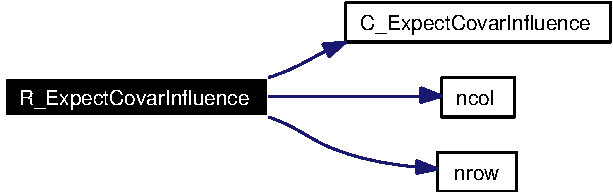
\includegraphics[width=164pt]{LinearStatistic_8c_6216ea560644c08002fb32756ae67dcc_cgraph}
\end{center}
\end{figure}
\hypertarget{LinearStatistic_8c_58fff8082d3ab197994a21a10c422353}{
\index{LinearStatistic.c@{LinearStatistic.c}!R\_\-ExpectCovarLinearStatistic@{R\_\-ExpectCovarLinearStatistic}}
\index{R\_\-ExpectCovarLinearStatistic@{R\_\-ExpectCovarLinearStatistic}!LinearStatistic.c@{LinearStatistic.c}}
\subsubsection{\setlength{\rightskip}{0pt plus 5cm}SEXP R\_\-ExpectCovarLinearStatistic (SEXP {\em x}, \/  SEXP {\em y}, \/  SEXP {\em weights}, \/  SEXP {\em expcovinf})}}
\label{LinearStatistic_8c_58fff8082d3ab197994a21a10c422353}


R-interface to C\_\-ExpectCovarLinearStatistic\par
 \begin{Desc}
\item[Parameters:]
\begin{description}
\item[{\em x}]values of the transformation \item[{\em y}]values of the influence function \item[{\em weights}]case weights \item[{\em expcovinf}]an object of class `ExpectCovarInfluence' \end{description}
\end{Desc}


Definition at line 306 of file LinearStatistic.c.

References C\_\-ExpectCovarLinearStatistic(), ncol(), nrow(), PL2\_\-covarianceSym, and PL2\_\-expectationSym.

Here is the call graph for this function:\nopagebreak
\begin{figure}[H]
\begin{center}
\leavevmode
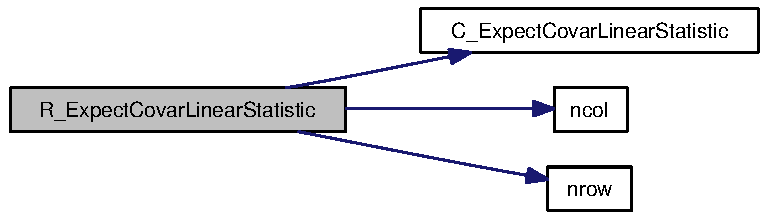
\includegraphics[width=242pt]{LinearStatistic_8c_58fff8082d3ab197994a21a10c422353_cgraph}
\end{center}
\end{figure}
\hypertarget{LinearStatistic_8c_732bfc8e1797d8953482aa31f9b43e5f}{
\index{LinearStatistic.c@{LinearStatistic.c}!R\_\-LinearStatistic@{R\_\-LinearStatistic}}
\index{R\_\-LinearStatistic@{R\_\-LinearStatistic}!LinearStatistic.c@{LinearStatistic.c}}
\subsubsection{\setlength{\rightskip}{0pt plus 5cm}SEXP R\_\-LinearStatistic (SEXP {\em x}, \/  SEXP {\em y}, \/  SEXP {\em weights})}}
\label{LinearStatistic_8c_732bfc8e1797d8953482aa31f9b43e5f}


R-interface to C\_\-LinearStatistic \par
 \begin{Desc}
\item[Parameters:]
\begin{description}
\item[{\em x}]values of the transformation \item[{\em y}]values of the influence function \item[{\em weights}]case weights \end{description}
\end{Desc}


Definition at line 59 of file LinearStatistic.c.

References C\_\-LinearStatistic(), ncol(), and nrow().

Here is the call graph for this function:\nopagebreak
\begin{figure}[H]
\begin{center}
\leavevmode
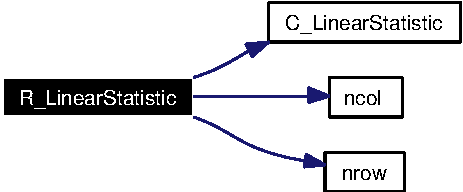
\includegraphics[width=130pt]{LinearStatistic_8c_732bfc8e1797d8953482aa31f9b43e5f_cgraph}
\end{center}
\end{figure}
\hypertarget{LinearStatistic_8c_be383bcae17e8b3a1d5740ec16a9817a}{
\index{LinearStatistic.c@{LinearStatistic.c}!R\_\-PermutedLinearStatistic@{R\_\-PermutedLinearStatistic}}
\index{R\_\-PermutedLinearStatistic@{R\_\-PermutedLinearStatistic}!LinearStatistic.c@{LinearStatistic.c}}
\subsubsection{\setlength{\rightskip}{0pt plus 5cm}SEXP R\_\-PermutedLinearStatistic (SEXP {\em x}, \/  SEXP {\em y}, \/  SEXP {\em indx}, \/  SEXP {\em perm})}}
\label{LinearStatistic_8c_be383bcae17e8b3a1d5740ec16a9817a}


Linear Statistic with permuted indices\par
 \begin{Desc}
\item[Parameters:]
\begin{description}
\item[{\em x}]values of the transformation \item[{\em y}]values of the influence function \item[{\em indx}]indices for the x-part \item[{\em perm}](permuted) indices for the y-part \end{description}
\end{Desc}


Definition at line 384 of file LinearStatistic.c.

References C\_\-PermutedLinearStatistic(), ncol(), and nrow().

Here is the call graph for this function:\nopagebreak
\begin{figure}[H]
\begin{center}
\leavevmode
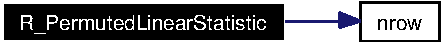
\includegraphics[width=172pt]{LinearStatistic_8c_be383bcae17e8b3a1d5740ec16a9817a_cgraph}
\end{center}
\end{figure}
